\documentclass{article}

\usepackage{fullpage}
\usepackage{tikz}
\usetikzlibrary{calc}
\usetikzlibrary{positioning}
\usepackage{capt-of}

\begin{document}
\thispagestyle{empty}
\begin{figure}[htp]
	\begin{center}
	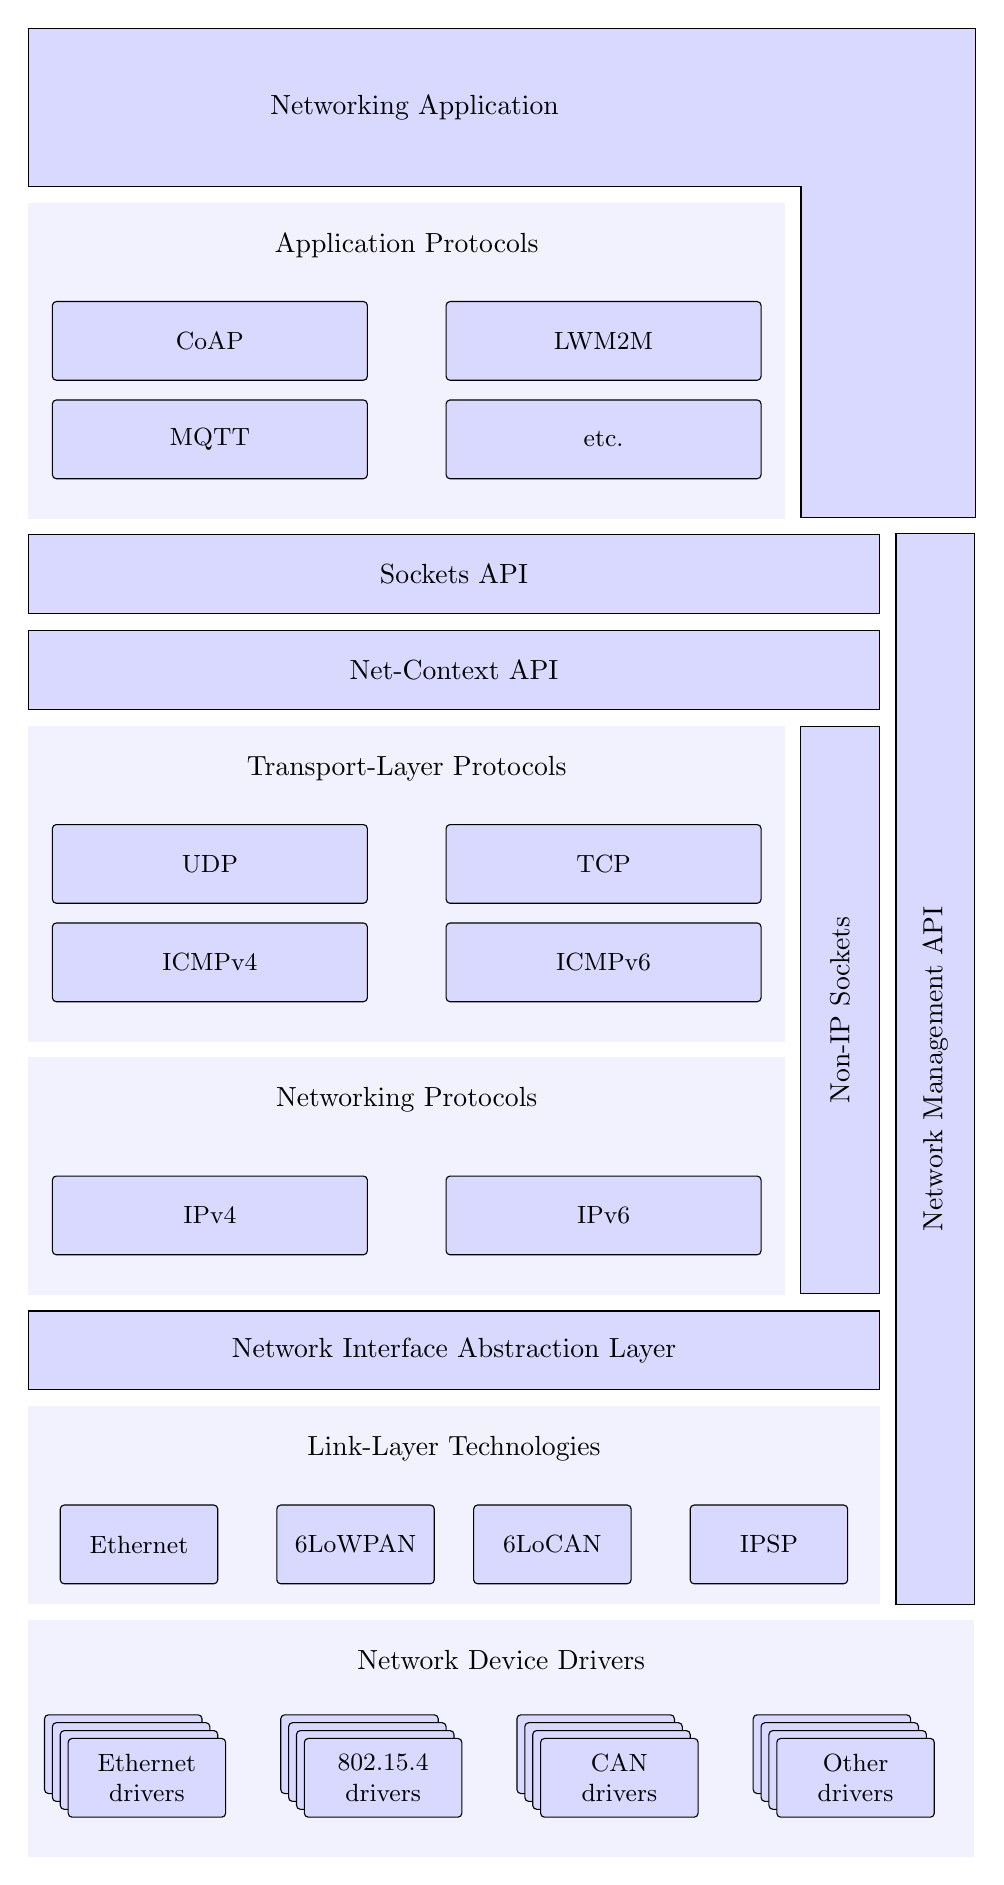
\begin{tikzpicture}[
		scale=1,
		every node/.append style={scale=1},
		layers/.style={
			fill=blue!5,
			rectangle,
			draw=blue!5,
			node distance=0.2cm},
		layers_dark/.style={
			draw=black,
			fill=blue!15,
			rectangle,
			node distance=0.2cm},
		layer_rot/.style={
			draw=black,
			fill=blue!15,
			rectangle},
		instance/.style={
			draw=black,
			rounded corners=0.05cm,
			fill=blue!15,
			rectangle, 
			minimum width=2cm,
			minimum height=1cm,
			align=center,
			font=\small},
		instance_wide/.style={
			draw=black,
			rounded corners=0.05cm,
			fill=blue!15,
			rectangle, 
			minimum width=4cm,
			minimum height=1cm,
			align=center,
			font=\small},
		]

		%App
		\node (app)[layers_dark, draw=blue!15, node distance=0cm, minimum width = 9.8cm, minimum height = 2cm] {Networking Application};
		\node (appbare)[layers_dark, draw=blue!15, node distance=0cm, right = of app.north east, anchor=north west, xshift=0cm, minimum width = 2.2cm, minimum height=6.2cm] {};
		\draw (app.north west) -- (appbare.north east) -- (appbare.south east) -- (appbare.south west) -- (app.south east) -- (app.south west) -- (app.north west);
	
		%Application Protocols
		\node (appprot)[layers,below = of app.south west,anchor=north west, minimum width = 9.6cm, minimum height = 4cm, text depth = 3cm] {Application Protocols};
		\foreach \approtocol/\x/\y in {CoAP/-2.5/0.75, LWM2M/2.5/0.75, MQTT/-2.5/-0.5, etc./2.5/-0.5}{
			\node at ($(appprot) + (\x cm, \y cm -0.5 cm)$) [instance_wide] {\approtocol};
		}
		
		%Sockets API
		\node (sockets)[layers_dark, below = of appprot.south west,anchor=north west, minimum width = 10.8cm, minimum height = 1cm] {Sockets API};

		%Net-context
		\node (netctx)[layers_dark, below = of sockets.south west,anchor=north west, minimum width = 10.8cm, minimum height = 1cm] {Net-Context API};
	
		%Transport-Layer Protocols
		\node (transp)[layers,below = of netctx.south west,anchor=north west, minimum width = 9.6cm, minimum height = 4cm, text depth = 3cm] {Transport-Layer Protocols};
		\foreach \tansport/\x/\y in {UDP/-2.5/0.75, TCP/2.5/0.75, ICMPv4/-2.5/-0.5, ICMPv6/2.5/-0.5}{
			\node at ($(transp) + (\x cm, \y cm -0.5 cm)$) [instance_wide] {\tansport};
		}

		%Networking Protocols
		\node (netw)[layers,below = of transp.south west,anchor=north west, minimum width = 9.6cm, minimum height = 3cm, text depth = 2cm] {Networking Protocols};
		\foreach \network/\x in {IPv4/-2.5, IPv6/2.5}{
			\node at ($(netw) + (\x cm, -0.5 cm)$) [instance_wide] {\network};
		}

		%Interface Abstraction
		\node (interf)[layers_dark, below = of netw.south west,anchor=north west, minimum width = 10.8cm, minimum height = 1cm] {Network Interface Abstraction Layer};

		%Non-IP Sockets
		\node at ($(netctx)!0.5!(interf) + (4.9cm ,0)$) [layer_rot, rotate=90, minimum width=7.2cm, minimum height=1cm] {Non-IP Sockets};

		%Link-Layer
		\node (linklayer)[layers, below = of interf.south west,anchor=north west, minimum width = 10.8cm, minimum height = 2.5cm, text depth = 1.5cm] {Link-Layer Technologies};
		\foreach \linklayer/\x in {Ethernet/-4, 6LoWPAN/-1.25, 6LoCAN/1.25, IPSP/4}{
			\node at ($(linklayer) + (\x cm, -0.5 cm)$) [instance] {\linklayer};
		}
		
		%Network drivers
		\node (net_drivers)[layers, below = of linklayer.south west,anchor=north west, minimum width = 12cm, minimum height = 3cm, text depth = 2cm] {Network Device Drivers};
		\foreach \driver/\x in {Ethernet/-4.5, 802.15.4/-1.5, CAN/1.5, Other/4.5}{
			\foreach \inst in {0.3,0.2,0.1}{
				\node at ($(net_drivers) + (\x cm - \inst cm, -0.5 cm + \inst cm)$) [instance] {};
			}
			\node at ($(net_drivers) + (\x cm, -0.5 cm)$) [instance] {\driver \\ drivers};
		}

		%Network Management API
		\node at ($(appbare.south east)!0.5!(net_drivers.north east) + (-0.5cm ,0)$) [layer_rot, rotate=90, minimum width=13.6cm, minimum height=1cm,] {Network Management API};

	\end{tikzpicture}
%	\caption{Zephyr Network Stack}
	\label{fig:zephyr_net_satck}
	\end{center}
\end{figure}
\end{document}
